\hypertarget{spinner_8cpp}{}\section{src/spinner.cpp File Reference}
\label{spinner_8cpp}\index{src/spinner.\+cpp@{src/spinner.\+cpp}}


This file implements a spinner to time a loop.  


{\ttfamily \#include $<$pthread.\+h$>$}\newline
{\ttfamily \#include $<$iostream$>$}\newline
{\ttfamily \#include $<$real\+\_\+time\+\_\+tools/spinner.\+hpp$>$}\newline
{\ttfamily \#include $<$real\+\_\+time\+\_\+tools/timer.\+hpp$>$}\newline
Include dependency graph for spinner.\+cpp\+:
\nopagebreak
\begin{figure}[H]
\begin{center}
\leavevmode
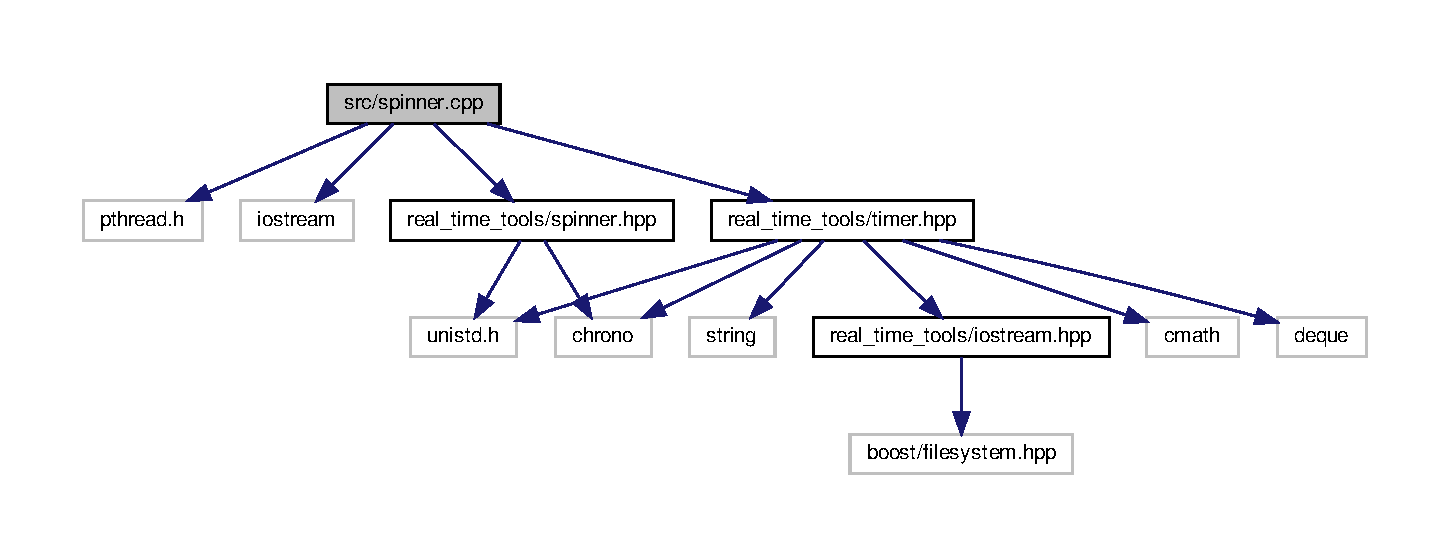
\includegraphics[width=350pt]{spinner_8cpp__incl}
\end{center}
\end{figure}


\subsection{Detailed Description}
This file implements a spinner to time a loop. 

\begin{DoxyAuthor}{Author}
Maximilien Naveau (\href{mailto:maximilien.naveau@gmail.com}{\tt maximilien.\+naveau@gmail.\+com}) license License B\+S\+D-\/3-\/\+Clause 
\end{DoxyAuthor}
\begin{DoxyCopyright}{Copyright}
Copyright (c) 2019, New York University and Max Planck Gesellschaft. 
\end{DoxyCopyright}
\begin{DoxyDate}{Date}
2019-\/05-\/22 
\end{DoxyDate}
